% 
\documentclass[a4paper]{article}
\usepackage[OT1]{fontenc}
\usepackage{Sweave}
	\renewcommand{\familydefault}{\sfdefault}
\begin{document}

\title{This is the title}
\author{eric}

\maketitle
%  The way to make Sweave function within Eclipse is to manually change the working directory
%	as described in the help forum entry at 
%	http://lists.r-forge.r-project.org/pipermail/statet-user/2008-June/000023.html
%	use triangle in upper right corner of Console at right!!  
%      must have an active R session before doing this, activate session is step 1
%  Rerun on 25 Nov 2010 using StatEt 0.9.1 and all appears to work (use run
% Sweave as task to produce resulting pdf result)

This is pretty trivial really.  Think about the possibility (remote) of using Sweave with Eclipse and StatET
for preparing the ObsEff final report (if all hangs together)
\begin{Schunk}
\begin{Soutput}
Call:
lm(formula = y ~ x)

Residuals:
      Min        1Q    Median        3Q       Max 
-0.456445 -0.223355 -0.002638  0.182185  0.478860 

Coefficients:
              Estimate Std. Error t value Pr(>|t|)    
(Intercept)  4.5073320  0.1355728  33.247   <2e-16 ***
x           -0.0007257  0.0113174  -0.064     0.95    
---
Signif. codes:  0 '***' 0.001 '**' 0.01 '*' 0.05 '.' 0.1 ' ' 1 

Residual standard error: 0.2918 on 18 degrees of freedom
Multiple R-squared: 0.0002284,	Adjusted R-squared: -0.05531 
F-statistic: 0.004112 on 1 and 18 DF,  p-value: 0.9496 
\end{Soutput}
\end{Schunk}

For my next trick, I'll try some nesting

\begin{Schunk}
\begin{Sinput}
> nothing <- numeric(200)
> for (i in 1:200) {
+     j <- sqrt(i)
+     z <- i^(1/3)
+     nothing[i] <- cos(z)
+ }
> plot(seq(1:200), nothing)
\end{Sinput}
\end{Schunk}
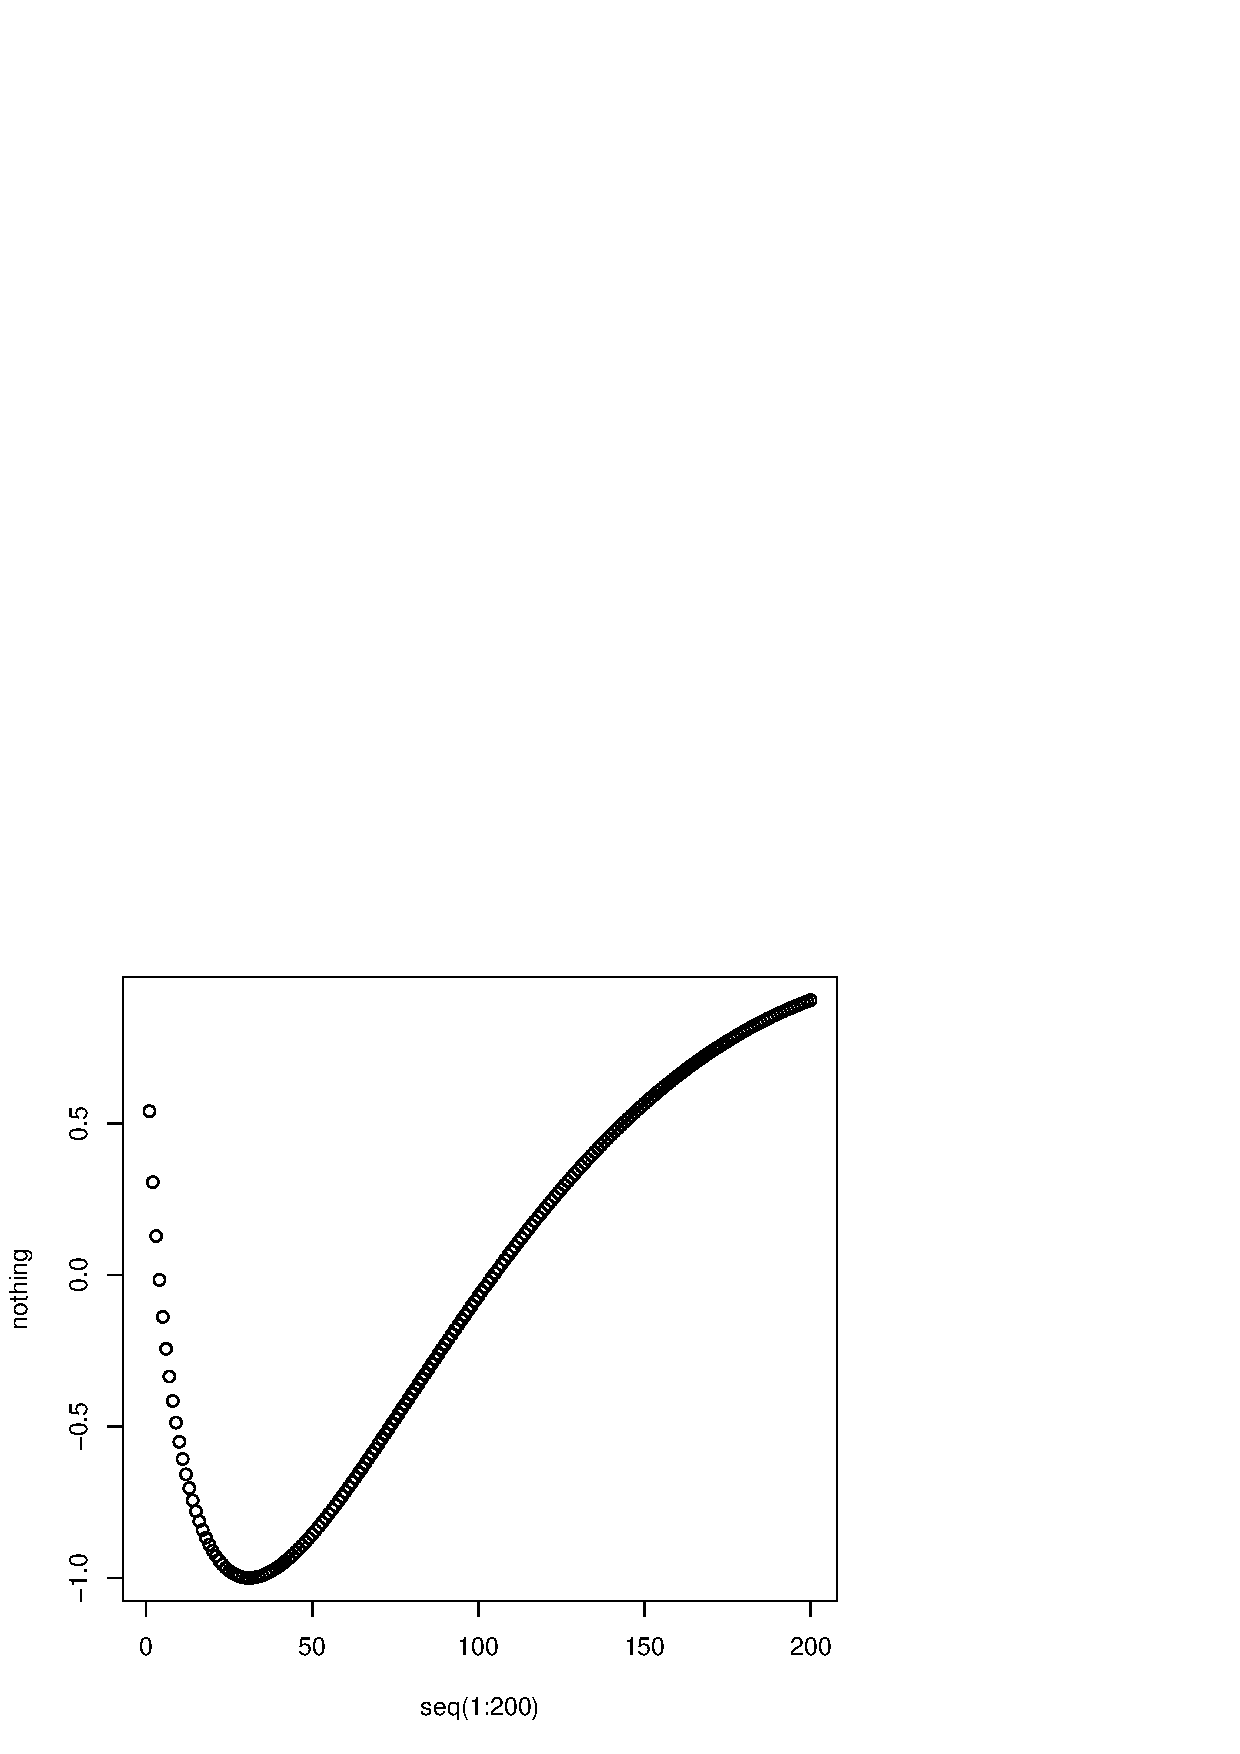
\includegraphics{first-sweave-b}
% comment

And we find that the coefficients are 4.51 
not very interesting.

And that is how it is, with gratuitous symbols $\delta \gamma \Leftarrow \Pi$.

And that is the conclusion of the \textbf{Observer Effectiveness} report.

\end{document}
